% Ember: research paper (NASA Space Apps Challenge 2026)
% Build: python scripts/build_paper.py   (draws figures/, writes numbers.tex, compiles this file)
% Every number traces to the cleaned NASA data: model scores to docs/methods/results.md
% (scripts/evaluate_methods.py), live fire-check examples to numbers.tex.
\documentclass[11pt,twocolumn]{article}

\usepackage[letterpaper,margin=0.75in,columnsep=0.3in]{geometry}
\usepackage[T1]{fontenc}
\usepackage[utf8]{inputenc}
\usepackage{lmodern}
\usepackage{microtype}
\usepackage{amsmath}
\usepackage{graphicx}
\usepackage{booktabs}
\usepackage{tabularx}
\usepackage[font=small,labelfont=bf,skip=4pt]{caption}
\usepackage{enumitem}
\usepackage[hidelinks]{hyperref}

\graphicspath{{figures/}}
\setlist{nosep,leftmargin=*}
\newcommand{\Otwo}{\ensuremath{\mathrm{O_2}}}
\newcommand{\COtwo}{\ensuremath{\mathrm{CO_2}}}
\newcommand{\pct}{\,\%}
% Generated by scripts/build_paper.py from the live fire check. Do not edit by hand.
\newcommand{\MoonZone}{estimated}
\newcommand{\MoonP}{38}
\newcommand{\MoonLow}{25}
\newcommand{\MoonHigh}{52}
\newcommand{\MoonPeak}{33}
\newcommand{\MoonGZone}{untested}
\newcommand{\PropZone}{untested}
\newcommand{\NextOtwo}{33.4}
\newcommand{\NextPsi}{14.7}
\newcommand{\NextFlow}{0.74}
\newcommand{\NextLow}{12}
\newcommand{\NextHigh}{96}
\newcommand{\MapFuel}{30\,\% butane}
\newcommand{\MapFlow}{1.38}
\newcommand{\MapMax}{49.3}
\newcommand{\MethCross}{29.7}


\title{\textbf{Will a Small Fire Keep Burning in Habitat Air?\\
Learning from NASA Microgravity Combustion Experiments}}
\author{Ember Team\\[2pt]
\normalsize NASA Space Apps Challenge 2026}
\date{November 2026}

\begin{document}

\twocolumn[
\begin{@twocolumnfalse}
\maketitle
\vspace{-1.2em}
\begin{abstract}
\noindent
Moon and Mars habitats are planned with more oxygen at lower pressure than the International Space Station
(for example 34\pct{} \Otwo{} at 8.2\,psi, against 21\pct{} at 14.7\,psi). In microgravity there is no
buoyant flow, so flammability data from Earth is a poor guide. We ask whether a small fire keeps burning under
such conditions, using only NASA's own experiments. We retrieved 19 experimental tables from NASA Physical
Sciences Informatics (1{,}903 rows) and cleaned them under a \emph{flag, never fix} rule (55 rows excluded,
1{,}848 retained). Two tables record whether the flame survived: gas-jet flames (CFI-G, 133 tests) and fuel
droplets (FLEX, 206 tests). We compared logistic regression, a random forest and a Gaussian process classifier
on whole test campaigns withheld from training, under a selection rule fixed in advance: beat a constant
baseline on both Brier score and log loss. The Gaussian process was selected for both questions
(AUC $0.830 \pm 0.032$ and $0.838 \pm 0.013$; Brier 0.123 against a baseline of 0.179, and 0.094 against
0.114). Every estimate carries a bootstrap range and is withheld outside the tested domain. A model-free test
supports the main finding: no gas flame stayed lit below 30\pct{} \Otwo{} (0 of 41, against 29 of 89 at
35--40\pct; Fisher exact $p = 5.4 \times 10^{-6}$). The data also reveals the most important gap: there are no
gas-jet tests with an outcome between 25\pct{} and 33\pct{} \Otwo, which is the Moon-base range.
\end{abstract}
\vspace{0.3em}
\noindent\textbf{Keywords:} microgravity combustion; spacecraft fire safety; exploration atmospheres;
Gaussian processes; grouped cross-validation; applicability domain.
\vspace{1.2em}
\end{@twocolumnfalse}
]

% =====================================================================================================
\section{Introduction}

Fire is one of the most serious hazards in a sealed spacecraft or surface habitat. The challenge brief for
this problem names cabin atmospheres of 30\pct{} oxygen or more at 10.2\,psi or less; our reference
Moon-base setting is 34\pct{} \Otwo{} at 8.2\,psi. A higher oxygen fraction makes fires easier to start and
sustain, and reduced gravity removes the buoyant flow that both feeds and cools a flame on Earth. A flame
in a habitat may therefore behave in ways that ground tests do not predict~\cite{nasa2015guide}.

NASA has run hundreds of combustion experiments on the International Space Station (ISS). The results are
public through the Physical Sciences Informatics (PSI) system~\cite{psi}, but they are spread over many
tables, each with its own format, outcome codes, free-text notes and errors. They have not been combined
into a form that answers an engineering question directly.

We address a narrow, practical question: \emph{for a given cabin atmosphere and fuel, did NASA observe a small
fire keep burning, and how certain can we be between and beyond its tests?} We test three hypotheses:
\begin{enumerate}[label=\textbf{H\arabic*.}]
  \item A higher oxygen percentage raises the probability that a flame keeps burning.
  \item Oxygen percentage predicts the outcome better than oxygen partial pressure.
  \item A model of the test conditions predicts outcomes on unseen test campaigns better than a constant
        baseline.
\end{enumerate}
Our contributions are (i) a reproducible, logged cleaning pipeline for 19 PSI tables; (ii) calibrated
classifiers validated on withheld campaigns, with an explicit applicability domain; (iii) model-free checks
of the main conclusion; and (iv) an open tool, \emph{Ember}, that exposes these results.

% =====================================================================================================
\section{Background}

Without gravity, hot combustion products do not rise, so oxygen reaches a flame only by diffusion or by
forced ventilation. Flame survival then depends on the flow speed in a non-monotonic way: at very low flow
the flame is starved of oxygen and quenches, and at high flow it is blown off. Between the two lies a
minimum oxygen level below which no flame survives~\cite{olson1991}. On Earth, buoyancy supplies a flow
of the order of 30\,cm/s at all times, which is why ground tests can mislead in both directions.

NASA materials testing found that flammability depends more on oxygen \emph{concentration} than on
equivalent partial pressure~\cite{harper2016}. This matters because exploration atmospheres combine a higher
oxygen fraction with a lower total pressure. If partial pressure governed flammability, the two changes
could cancel out.

% =====================================================================================================
\section{Data}
\label{sec:data}

All measured data comes from NASA PSI~\cite{psi}. A fetch script pins a SHA-256 checksum for each file, so a
changed or corrupted table is detected. Table~\ref{tab:sources} lists the sources. Only two tables record
both the test conditions and whether the flame survived, so only these can train a model:

\paragraph{CFI-G (PSI-159), gas-jet flames.} A small tube releases gaseous fuel (ethane, propane or
butane, sometimes diluted to 30\pct{} or 50\pct{} with nitrogen) into an atmosphere of chosen oxygen and
pressure. The outcome is \emph{stayed lit} until the fuel was stopped, or \emph{went out on its own}. There
are 133 tests (31 stayed lit), spanning 18--40\pct{} \Otwo{} and 7.4--44\,psi. This is a model of a small gas
leak that ignites.

\paragraph{FLEX (PSI-69), fuel droplets.} A single drop of heptane or methanol (1.1--4.7\,mm) is ignited
and burns as a sphere. The outcome is \emph{burned to the end} or \emph{extinguished with fuel left}. The
table also records the burning-rate constant $K$ ($d^2$ law) and the drop diameter at extinction. There are
206 tests (27 burned to the end), spanning 12--34\pct{} \Otwo, 10--45\,psi, up to 70\pct{} \COtwo{} and up to
45\pct{} helium. This is a model of a spilled liquid that ignites.

The remaining tables either lack a per-test outcome or cabin pressure (solid materials), are daily
summaries (ACME, E-FIELD, SLICE), or measure smoke (SAME). They serve only as evidence of what was and was
not tested. One non-NASA source, ZARM drop-tower flame-spread data~\cite{zarm}, is kept apart and trains no
model.

\begin{table}[t]
\centering
\caption{The 19 NASA PSI tables used (1{,}903 rows read, 1{,}848 retained). M: trains a model; E: evidence
and coverage only.}
\label{tab:sources}
\small
\begin{tabularx}{\columnwidth}{@{}l X c@{}}
\toprule
Group & Experiments (PSI study) & Role \\
\midrule
Droplets & FLEX (69); CFI (39); FLEX-2 (68) & M / E \\
Gas flames & CFI-G (159); ACME (10, 20, 21, 23); E-FIELD (22); SPICE (107); SLICE (106) & M / E \\
Solids & BASS-II (25); BASS (26); SAFFIRE-1/2/3 (98--100) & E \\
Smoke & SAME (102); SAME-R (101) & E \\
\bottomrule
\end{tabularx}
\end{table}

% =====================================================================================================
\section{Methods}

\subsection{Data cleaning}

The governing rule is \emph{flag, never silently fix}. A row is removed only when it is provably wrong;
anything that merely looks odd is kept and flagged with a written reason, and every decision is logged.
Checks run before unit conversion, so a bad value is never converted into a believable one. Values read
from free-text notes are marked \emph{derived}, and a missing material or fuel is never guessed. Statistical
outliers are not deleted: with only 27--31 positive outcomes per model, an extreme test is often the most
informative one. Table~\ref{tab:cleaning} summarises the rules.

\begin{table}[t]
\centering
\caption{Cleaning rules and the number of rows each caught.}
\label{tab:cleaning}
\small
\begin{tabularx}{\columnwidth}{@{}X l r@{}}
\toprule
Rule (example) & Action & Rows \\
\midrule
Impossible value (FLEX-114: 0\,mmHg) & excluded & 11 \\
Duplicate test identifier & excluded & 44 \\
Implausible (thickness ``37\,mm'') & flagged & 7 \\
Gas fractions do not sum to 100\pct & flagged & 6 \\
Extinction diameter $>$ initial & flagged & 1 \\
Missing outcome & flagged & 131 \\
\bottomrule
\end{tabularx}
\end{table}

\subsection{Model inputs}

Gas-jet inputs are oxygen percentage, pressure, fuel flow, the number of carbon atoms in the fuel (2, 3 or 4)
and the fuel's share of the jet (0.3, 0.5 or 1). Describing the fuel by two physical numbers instead of six
labels lets the model share information between fuels. Droplet inputs are oxygen percentage, pressure,
initial diameter, fuel, \COtwo{} percentage and helium percentage. Inputs are standardised within each
training fold only. With about 4--5 positive outcomes per input~\cite{riley2019}, we kept the inputs few.
We did not rebalance the classes, because imbalance corrections distort predicted
probabilities~\cite{goorbergh2022}. We did not impute: a row missing a required input is left out of that
model.

\subsection{Models and selection rule}

Each question is a supervised binary classification whose output is a probability $\hat p_i$. We compared
logistic regression; a random forest (400 trees, minimum leaf size 3); and a Gaussian process (GP)
classifier~\cite{rasmussen2006} with the kernel
\begin{equation}
k(\mathbf{x}, \mathbf{x}') = \sigma^2 \exp\!\Big(-\tfrac{1}{2}\sum_{j} \frac{(x_j - x'_j)^2}{\ell_j^2}\Big),
\end{equation}
which learns one length scale $\ell_j$ per input. The reference is a constant baseline,
$\hat p_i = \bar y$ (23\pct{} for gas jets and 13\pct{} for droplets). Models are scored by the Brier
score~\cite{brier1950} and the log loss,
\begin{align}
\mathrm{BS} &= \frac{1}{n}\sum_{i=1}^{n} (\hat p_i - y_i)^2, \\
\mathrm{LL} &= -\frac{1}{n}\sum_{i=1}^{n} \big[y_i \ln \hat p_i + (1-y_i)\ln(1-\hat p_i)\big],
\end{align}
together with the area under the ROC curve (AUC) and the calibration slope. The selection rule was fixed
before any comparison: a model is usable only if it beats the baseline on \emph{both} BS and LL on unseen
campaigns, and the usable model with the lowest LL is chosen. The droplet burning-rate constant, extinction
diameter and burn time are modelled with the same model families as regressors and compared on mean
absolute error (MAE). All models use scikit-learn~\cite{pedregosa2011}.

\subsection{Validation design}

NASA ran its tests in campaigns, and tests within a campaign are near-repeats. Random splits therefore
overstate skill: $k$-nearest neighbours on FLEX scored AUC 0.89 with random splits but 0.71 with campaigns
withheld. We use grouped 5-fold cross-validation with the campaign as the group (11 campaigns for gas jets,
12 for droplets), repeated over 10 different campaign partitions, and report the mean and spread. We do not
use accuracy: always predicting ``extinguished'' already scores 87\pct{} on droplets.

\subsection{Uncertainty and applicability domain}

The selected model is refitted on 15 campaign-bootstrap samples, in which whole campaigns are drawn with
replacement. The 10th--90th percentile of their predictions is the range reported with each estimate.
Regression intervals (90\pct) are taken from the empirical errors on unseen campaigns.

Following OECD QSAR principle~3~\cite{oecd2007}, each request $\mathbf{x}$ is assigned to a zone by its
standardised distance to tests of the \emph{same fuel},
\begin{equation}
d(\mathbf{x}, \mathbf{x}_k) = \Big[\sum_j \Big(\frac{x_j - x_{kj}}{s_j}\Big)^2\Big]^{1/2},
\end{equation}
where $s_j$ is the spread of input $j$ in the training data. The thresholds come from the data's own
nearest-neighbour distances. A request is \emph{tested} if it lies within the median nearest-neighbour
distance, and the real tests then answer. It is \emph{estimated} if it lies inside every tested range and
within twice the 95th percentile of the mean 5-nearest-neighbour distance. Otherwise, or at any gravity
other than microgravity, it is \emph{untested}, and no number is produced. The 15 refits also form a
committee: where they disagree most, within conditions the hardware has already reached, the tool proposes
the next experiment (query by committee~\cite{seung1992}).

\subsection{Model-free checks}

The main conclusion is also tested directly on the data, with no model involved. We check
\emph{significance} with Fisher's exact test, comparing the share of gas flames that stayed lit below
30\pct{} and at 35--40\pct{} \Otwo. We check \emph{stability} by recomputing the lowest oxygen at which a flame
stayed lit with each campaign left out in turn. We check \emph{coverage} by counting the tests in the
25--33\pct{} \Otwo{} band.

\subsection{Exploratory grouping}

As an unsupervised check, a Gaussian mixture is fitted to the standardised test conditions without the
outcome. The number of groups (2--6) is chosen by the Bayesian information criterion~\cite{schwarz1978}, and
the groups are compared with NASA's campaigns using the adjusted Rand index (ARI)~\cite{hubert1985}.

\subsection{Illustrative flame simulator}

Ember's flame simulator gives visual intuition only and never produces fire-check estimates. A flame burns
when $X_{\Otwo} \ge X_{\lim}$, with
\begin{align}
u_{\mathrm{eff}} &= \sqrt{u^2 + (30\sqrt{g})^2 + u_d^2}, \\
X_{\lim} &= \Big[X_{\min} + k \ln^2\!\frac{u_{\mathrm{eff}}}{u^*}\Big]\Big(\frac{14.7}{P}\Big)^{n},
\end{align}
where $u$ is the forced flow (cm/s), $g$ the gravity in Earth units, $u_d = 0.3$\,cm/s a diffusion floor and
$P$ the pressure in psi. Below $u^*$ the flame quenches; above it the flame is blown off, following the
flammability boundary of~\cite{olson1991}. Six literature anchor cases are checked automatically. For
example, cotton-fibreglass fabric at 0\,$g$, 21\pct{} \Otwo{} and 20\,cm/s must spread at
$1.8 \pm 0.15$\,mm/s, as observed in Saffire-I.

% =====================================================================================================
\section{Results}

\subsection{Oxygen threshold and coverage gap}

\begin{figure}[t]
\centering
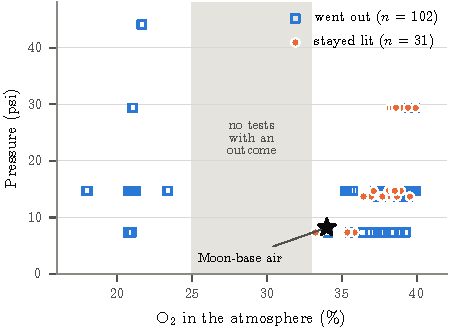
\includegraphics[width=\columnwidth]{fig1_gas_outcomes.pdf}
\caption{Every CFI-G gas-jet test with a recorded outcome. Orange circles stayed lit; blue squares went out
on their own. The grey band (25--33\pct{} \Otwo) contains no tests with an outcome. The star marks the
Moon-base setting.}
\label{fig:gas}
\end{figure}

No gas flame stayed lit below 30\pct{} \Otwo: 0 of 41 tests, against 29 of 89 at 35--40\pct{} (Fisher exact
$p = 5.4 \times 10^{-6}$). The lowest oxygen at which a flame stayed lit is 33.2\pct. It stays between
33.2\pct{} and 35.4\pct{} whichever campaign is left out, so no single campaign drives it. However, there are
\emph{no} gas-jet tests with an outcome between 25\pct{} and 33\pct{} \Otwo{} (Fig.~\ref{fig:gas}). The
supported statement is therefore ``no flame stayed lit below 30\pct{} in these tests'', not ``flames need
33\pct{} oxygen''. This supports H1 and identifies the most important gap in the data.

\subsection{Model comparison}

\begin{table*}[t]
\centering
\caption{Scores on withheld campaigns: mean $\pm$ spread over 10 campaign partitions. BS: Brier score
(lower is better); slope: calibration slope (1 is ideal). $^\dagger$Does not beat the baseline.}
\label{tab:models}
\small
\begin{tabular}{@{}l ccc ccc@{}}
\toprule
& \multicolumn{3}{c}{Gas jets (CFI-G, $n = 133$)} & \multicolumn{3}{c}{Droplets (FLEX, $n = 206$)} \\
\cmidrule(lr){2-4} \cmidrule(l){5-7}
Model & AUC & BS & Slope & AUC & BS & Slope \\
\midrule
Baseline (constant) & 0.500 & 0.179 & -- & 0.500 & 0.114 & -- \\
Logistic regression & $0.815 \pm 0.023$ & 0.132 & 0.86 & $0.757 \pm 0.029$ & 0.115$^\dagger$ & 0.53 \\
Random forest & $0.809 \pm 0.031$ & 0.130 & 1.15 & $0.760 \pm 0.016$ & 0.101 & 0.95 \\
\textbf{Gaussian process} & $\mathbf{0.830 \pm 0.032}$ & \textbf{0.123} & \textbf{1.00} &
$\mathbf{0.838 \pm 0.013}$ & \textbf{0.094} & \textbf{0.90} \\
\bottomrule
\end{tabular}
\end{table*}

\begin{figure}[t]
\centering
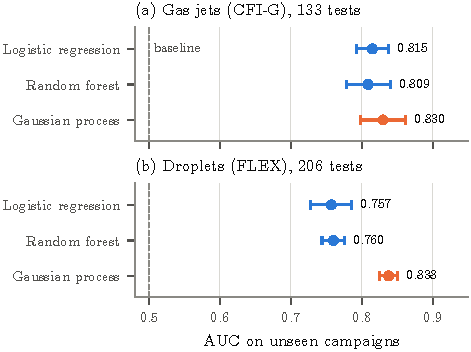
\includegraphics[width=\columnwidth]{fig2_models.pdf}
\caption{AUC on unseen campaigns (mean and spread over 10 partitions). The dashed line is the constant
baseline. The Gaussian process (orange) was selected by the pre-set rule for both questions.}
\label{fig:models}
\end{figure}

All three models beat the baseline on gas jets. On droplets, logistic regression does not
(BS 0.115 against 0.114; Table~\ref{tab:models}). The GP is selected for both questions. It lowers the Brier
score by 31\pct{} (gas jets) and 18\pct{} (droplets) relative to the baseline, and it is well calibrated
(slopes 1.00 and 0.90). For droplets its lead is clear: about 0.08 AUC, against a spread of 0.01--0.03
between partitions (Fig.~\ref{fig:models}). For gas jets the three models lie within about 0.02 AUC, the size
of that spread, so we claim ``best of three close candidates'', not ``optimal''. H3 is supported. Every
model's predicted probability rose with oxygen in 92--100\pct{} of steps along the oxygen axis, consistent
with combustion physics.

\subsection{Preprocessing ablations}

\begin{table}[t]
\centering
\caption{Ablations (logistic regression unless noted), mean over 10 campaign partitions.}
\label{tab:ablation}
\small
\begin{tabularx}{\columnwidth}{@{}X c c@{}}
\toprule
Choice & AUC & BS \\
\midrule
Gas: fuel as C atoms + share (used) & 0.815 & 0.132 \\
Gas: fuel as 6 labels & 0.766 & 0.146 \\
Gas: \Otwo{} partial pressure & 0.649 & 0.197 \\
Gas: add 139 inverse flames & 0.532 & 0.205 \\
Gas: balanced class weights & 0.821 & 0.168 \\
Drops: \Otwo{} partial pressure & 0.692 & 0.115 \\
Drops: balanced class weights & 0.741 & 0.232 \\
Drops, GP: flagged rows removed & 0.830 & 0.095 \\
Drops, GP: all rows (used) & 0.838 & 0.094 \\
\bottomrule
\end{tabularx}
\end{table}

Oxygen \emph{percentage} predicts far better than oxygen partial pressure for both questions
(Table~\ref{tab:ablation}: AUC 0.815 against 0.649 for gas jets, and 0.757 against 0.692 for droplets). This
supports H2 and agrees with NASA materials testing~\cite{harper2016}. In practice, lowering cabin pressure
does not cancel the effect of raising the oxygen fraction. Adding inverse flames, which involve different
physics, reduces the model to chance level. Class weighting leaves the ranking unchanged but roughly doubles
the droplet Brier score. Removing the six flagged FLEX rows changes nothing material.

\subsection{What the models learned}

\begin{figure*}[t]
\centering
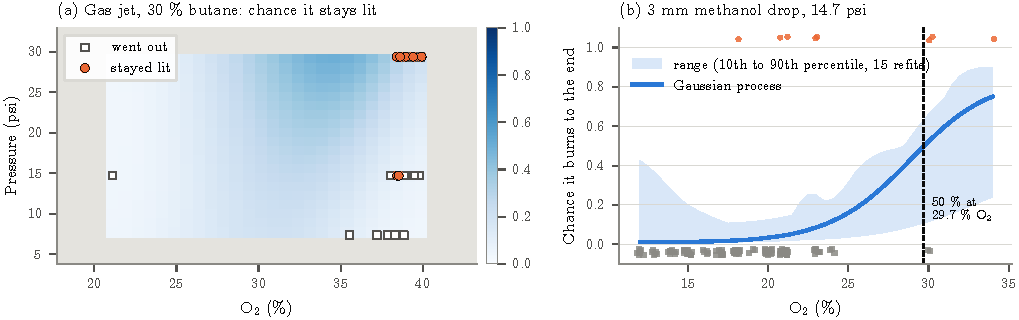
\includegraphics[width=\textwidth]{fig3_learned.pdf}
\caption{(a) GP probability that a \MapFuel{} jet stays lit, over oxygen and pressure, with fuel flow held
at its median (\MapFlow\,mg/s). Grey cells are \emph{untested}, where no number is given; the probability
stays below 50\pct{} everywhere on this map (maximum \MapMax\pct). (b) Probability that a 3\,mm methanol drop
at 14.7\,psi burns to the end, with the range of the 15 campaign-bootstrap refits. Dots are NASA methanol
tests: orange (top) burned to the end; grey (bottom) were extinguished with fuel left.}
\label{fig:learned}
\end{figure*}

For a 3\,mm methanol drop at 14.7\,psi, the probability of burning to the end passes 50\pct{} at about
\MethCross\pct{} \Otwo{} (Fig.~\ref{fig:learned}b), and the refits begin to disagree from about 28.5\pct. The
regressions also beat their baselines on unseen campaigns. The MAE of the droplet $K$ is 0.059 against
0.112\,mm$^2$/s, and the MAE of the extinction diameter is 0.27 against 0.80\,mm. Their 90\pct{} intervals
covered 89.9\pct{} of unseen tests, as intended.

The unsupervised grouping found 5 condition groups for gas jets and 6 for droplets, separated mainly by
oxygen and diluent. In the two gas-jet groups near 21\pct{} \Otwo, no flame stayed lit; in the three groups
near 37--39\pct, between 6\pct{} and 56\pct{} did. Agreement with NASA's campaigns was low to moderate
(ARI 0.16 and 0.34), so the structure does not simply reproduce the test schedule.

\subsection{Case study: Moon-base atmosphere}

A 30\pct{} ethane jet at 34\pct{} \Otwo, 8.2\,psi and 1\,mg/s in microgravity falls in the \emph{\MoonZone}
zone, and the GP gives a probability of \MoonP\pct{} that it stays lit (range \MoonLow--\MoonHigh\pct). At
these settings the probability peaks near \MoonPeak\pct{} \Otwo{} and then falls, so the tool flags that part
of the curve for caution. The decline reflects several nearby tests that went out at 38--40\pct{} \Otwo,
probably for reasons other than oxygen. The same request at lunar gravity (0.166\,$g$) is
\emph{\MoonGZone}, and no number is given. Pure propane at 8.2\,psi is also \emph{\PropZone}, because NASA
tested propane only at 13.7--14.7\,psi. The committee instead proposes a test at \NextOtwo\pct{} \Otwo,
\NextPsi\,psi and \NextFlow\,mg/s, where the refits disagree from \NextLow\pct{} to \NextHigh\pct. This is
the intended behaviour: an estimate where the data supports one, and a concrete next experiment where it
does not.

% =====================================================================================================
\section{Discussion}

\subsection{Interpretation}

The results support all three hypotheses. Oxygen percentage is the strongest driver of whether a small
flame survives in microgravity, and a lower pressure does not offset it. This matters for exploration
atmospheres, which combine both changes. The main result holds without any model; the models add
calibrated probabilities, uncertainty ranges and an explicit refusal outside the data.

\subsection{Limitations}

Gas jets and droplets stand in for a gas leak and a liquid spill. The main cabin hazard, burning solids such
as fabric, plastic and wiring, has no model, because the solid-material tables do not record pressure and
outcome together. All outcome data comes from microgravity, so partial gravity (Moon 0.166\,$g$, Mars
0.38\,$g$) is untested, and the tool refuses it. With 31 and 27 positive outcomes these are small-data
models, and for gas jets the choice among them is within noise. The simulator still uses its literature
default parameters: its fitting routine needs at least four verified solid-fuel points, and none has been
verified yet. The ZARM drop-tower data (thin acrylic spreading $2.6\times$ faster at 35.8\pct{} \Otwo{} than
in Earth air) agrees with the direction of the oxygen effect, but it uses a different fuel and a different
measurement. It therefore confirms the direction, not the values.

\subsection{Future work}

The most useful next steps are experimental: gas-jet tests between 25\pct{} and 33\pct{} \Otwo, any
partial-gravity combustion tests, and solid-material tests that record pressure and outcome. Review of
selected predictions by a combustion expert is the next validation step.

% =====================================================================================================
\section{Conclusion}

We cleaned NASA's microgravity combustion tables under strict, logged rules and validated models on test
campaigns they never saw. This turned scattered experiments into calibrated, traceable answers to a
practical question. In these tests, gas flames needed high oxygen to stay lit, oxygen percentage mattered
more than partial pressure, and the Moon-base oxygen range has not been tested. Ember reports a number only
where NASA's tests support one. Elsewhere it shows the nearest real tests and the experiment that would be
most informative.

\section*{Data and Code Availability}

All data are public NASA PSI tables~\cite{psi}. From a clean checkout, \texttt{python run.py ingest all}
loads and cleans the tables and trains the models; \texttt{python scripts/evaluate\_methods.py} regenerates
every score; \texttt{python scripts/build\_paper.py} regenerates the figures and this paper; and
\texttt{python run.py start} runs the tool. No API keys or log-in are required.

% =====================================================================================================
\small
\begin{thebibliography}{99}
\setlength{\itemsep}{1pt}

\bibitem{brier1950}
G.~W. Brier.
\newblock Verification of forecasts expressed in terms of probability.
\newblock \emph{Monthly Weather Review}, 78(1):1--3, 1950.

\bibitem{goorbergh2022}
R.~van~den Goorbergh, M.~van Smeden, D.~Timmerman, and B.~Van~Calster.
\newblock The harm of class imbalance corrections for risk prediction models.
\newblock \emph{Journal of the American Medical Informatics Association}, 29(9):1525--1534, 2022.

\bibitem{harper2016}
S.~A. Harper et~al.
\newblock Oxygen concentration versus partial pressure in materials flammability.
\newblock NASA White Sands Test Facility, NTRS 20160004937, 2016.

\bibitem{hubert1985}
L.~Hubert and P.~Arabie.
\newblock Comparing partitions.
\newblock \emph{Journal of Classification}, 2(1):193--218, 1985.

\bibitem{nasa2015guide}
NASA.
\newblock \emph{A Researcher's Guide to: Combustion Science}.
\newblock International Space Station Program Science Office, 2015.

\bibitem{psi}
NASA Physical Sciences Informatics.
\newblock Experiment data sets PSI-10, 20--23, 25, 26, 39, 68, 69, 98--102, 106, 107 and 159.
\newblock \url{https://psi.nasa.gov}.

\bibitem{oecd2007}
OECD.
\newblock \emph{Guidance Document on the Validation of (Quantitative) Structure-Activity Relationship
[(Q)SAR] Models}.
\newblock OECD Publishing, Paris, 2007.

\bibitem{olson1991}
S.~L. Olson.
\newblock Mechanisms of microgravity flame spread over a thin solid fuel: oxygen and opposed flow effects.
\newblock \emph{Combustion Science and Technology}, 76(4--6):233--249, 1991.

\bibitem{pedregosa2011}
F.~Pedregosa et~al.
\newblock Scikit-learn: Machine learning in Python.
\newblock \emph{Journal of Machine Learning Research}, 12:2825--2830, 2011.

\bibitem{rasmussen2006}
C.~E. Rasmussen and C.~K.~I. Williams.
\newblock \emph{Gaussian Processes for Machine Learning}.
\newblock MIT Press, 2006.

\bibitem{riley2019}
R.~D. Riley et~al.
\newblock Minimum sample size for developing a multivariable prediction model: Part II, binary and
time-to-event outcomes.
\newblock \emph{Statistics in Medicine}, 38(7):1276--1296, 2019.

\bibitem{schwarz1978}
G.~Schwarz.
\newblock Estimating the dimension of a model.
\newblock \emph{The Annals of Statistics}, 6(2):461--464, 1978.

\bibitem{seung1992}
H.~S. Seung, M.~Opper, and H.~Sompolinsky.
\newblock Query by committee.
\newblock In \emph{Proceedings of the Fifth Annual Workshop on Computational Learning Theory}, pages
287--294, 1992.

\bibitem{zarm}
ZARM drop-tower flame-spread measurements.
\newblock Zenodo, doi:10.5281/zenodo.18479713, CC BY-NC 4.0, 2026.

\end{thebibliography}

\end{document}
